\documentclass[]{scrartcl}
\usepackage{amsmath}
\usepackage{graphicx}

\usepackage{xcolor}
\definecolor{maroon}{cmyk}{0, 0.87, 0.68, 0.32}
\definecolor{halfgray}{gray}{0.55}
\definecolor{ipython-frame}{RGB}{207, 207, 207}
\definecolor{ipython-bg}{RGB}{247, 247, 247}
\definecolor{ipython-red}{RGB}{186, 33, 33}
\definecolor{ipython-green}{RGB}{0, 128, 0}
\definecolor{ipython-cyan}{RGB}{64, 128, 128}
\definecolor{ipython-purple}{RGB}{170, 34, 255}

\usepackage{listings}
\lstdefinelanguage{iPython}{
	morekeywords={access,and,del,except,exec,in,is,lambda,not,or,raise},
	morekeywords=[2]{for,print,abs,all,any,basestring,bin,bool,bytearray,callable,chr,classmethod,cmp,compile,complex,delattr,dict,dir,divmod,enumerate,eval,execfile,file,filter,float,format,frozenset,getattr,globals,hasattr,hash,help,hex,id,input,int,isinstance,issubclass,iter,len,list,locals,long,map,max,memoryview,min,next,object,oct,open,ord,pow,property,range,reduce,reload,repr,reversed,round,set,setattr,slice,sorted,staticmethod,str,sum,super,tuple,type,unichr,unicode,vars,xrange,zip,apply,buffer,coerce,intern,elif,else,if,continue,break,while,class,def,return,try,except,import,finally,try,except,from,global,pass, True, False},
	sensitive=true,
	morecomment=[l]\#,%
	morestring=[b]',%
	morestring=[b]",%
	moredelim=**[is][\color{black}]{@@}{@@},
	%%
	%morestring=[s]{'''}{'''},% used for documentation text (mulitiline strings)
	%morestring=[s]{"""}{"""},% added by Philipp Matthias Hahn
	%%
	%morestring=[s]{r'}{'},% `raw' strings
	%morestring=[s]{r"}{"},%
	%morestring=[s]{r'''}{'''},%
	%morestring=[s]{r"""}{"""},%
	%morestring=[s]{u'}{'},% unicode strings
	%morestring=[s]{u"}{"},%
	%morestring=[s]{u'''}{'''},%
	%morestring=[s]{u"""}{"""}%
	%
	% {replace}{replacement}{lenght of replace}
	% *{-}{-}{1} will not replace in comments and so on
	%literate=
	%{\%}{{{\color{ipython-purple}+}}}1,
	%{á}{{\'a}}1 {é}{{\'e}}1 {í}{{\'i}}1 {ó}{{\'o}}1 {ú}{{\'u}}1,
	%{Á}{{\'A}}1 {É}{{\'E}}1 {Í}{{\'I}}1 {Ó}{{\'O}}1 {Ú}{{\'U}}1
	%{à}{{\`a}}1 {è}{{\`e}}1 {ì}{{\`i}}1 {ò}{{\`o}}1 {ù}{{\`u}}1
	%{À}{{\`A}}1 {È}{{\'E}}1 {Ì}{{\`I}}1 {Ò}{{\`O}}1 {Ù}{{\`U}}1
	%{ä}{{\"a}}1 {ë}{{\"e}}1 {ï}{{\"i}}1 {ö}{{\"o}}1 {ü}{{\"u}}1
	%{Ä}{{\"A}}1 {Ë}{{\"E}}1 {Ï}{{\"I}}1 {Ö}{{\"O}}1 {Ü}{{\"U}}1
	%{â}{{\^a}}1 {ê}{{\^e}}1 {î}{{\^i}}1 {ô}{{\^o}}1 {û}{{\^u}}1
	%{Â}{{\^A}}1 {Ê}{{\^E}}1 {Î}{{\^I}}1 {Ô}{{\^O}}1 {Û}{{\^U}}1
	%{œ}{{\oe}}1 {Œ}{{\OE}}1 {æ}{{\ae}}1 {Æ}{{\AE}}1 {ß}{{\ss}}1
	%{ç}{{\c c}}1 {Ç}{{\c C}}1 {ø}{{\o}}1 {å}{{\r a}}1 {Å}{{\r A}}1
	%{€}{{\EUR}}1 {£}{{\pounds}}1
	%
	%{^}{{{\color{ipython_purple}\^{}}}}1
	%{=}{{{\color{ipython_purple}=}}}1
	%%
	%*{-}{{{\color{ipython_purple}-}}}1
	%{*}{{{\color{ipython_purple}$^\ast$}}}1
	%{/}{{{\color{ipython_purple}/}}}1%%
	%{+=}{{{+=}}}1
	%{-=}{{{-=}}}1
	%{*=}{{{$^\ast$=}}}1
	%{/=}{{{/=}}}1,
	%
	identifierstyle=\color{black}\footnotesize\ttfamily,
	commentstyle=\color{ipython-cyan}\footnotesize\itshape\ttfamily,
	stringstyle=\color{ipython-red}\footnotesize\ttfamily,
	keepspaces=true,
	showspaces=false,
	showstringspaces=false,
	rulecolor=\color{ipython-frame},
	frame=single,
	frameround={t}{t}{t}{t},
	%framexleftmargin=6mm,
	%numbers=left,
	%numberstyle=\color{ipython-cyan},
	backgroundcolor=\color{ipython-bg},
	%   extendedchars=true,
	basicstyle=\footnotesize\ttfamily,
	keywordstyle=[2]\color{ipython-green}\bfseries\footnotesize\ttfamily, 
	keywordstyle=\color{ipython-purple}\bfseries\footnotesize\ttfamily
}

\lstdefinelanguage{iOutput} {
	sensitive=true,
	identifierstyle=\color{black}\small\ttfamily,
	stringstyle=\color{ipython-red}\small\ttfamily,
	keepspaces=true,
	showspaces=false,
	showstringspaces=false,
	rulecolor=\color{ipython-frame},
	%frame=single,
	%frameround={t}{t}{t}{t},
	%backgroundcolor=\color{ipython-bg},
	basicstyle=\small\ttfamily,
}

\lstnewenvironment{ipython}[1][]{\lstset{language=iPython,mathescape=true,escapeinside={*@}{@*}}%
}{%
}

\lstnewenvironment{ioutput}[1][]{\lstset{language=iOutput,mathescape=true,escapeinside={*@}{@*}}%
}{%
}

\title{AoC Technicalities}
\author{}

\begin{document}

\maketitle

\section{Year 2023}

\subsection{Day 5 - Schoelace Formula}
\subsubsection{Schoelace Formula}

Suppose the polygon $P$ has vertices $(x_1, y_1)$, $(x_2, y_2)$, ... , $(x_n, y_n)$, listed in clockwise order. Then the area ($A$) of $P$ is

\begin{equation}
A = \cfrac{1}{2} \left|(x_1y_2 + x_2y_3 + \cdots + x_ny_1) - (y_1x_2 + y_2x_3 + \cdots + y_nx_1) \right|
\end{equation}
You can also go counter-clockwise order, as long as you find the absolute value of the answer.

The \emph{Shoelace Theorem} gets its name because if one lists the coordinates in a column,

\begin{align*} 
	(x_1 &, y_1) \\ 
	(x_2 &, y_2) \\ & \vdots \\ (x_n &, y_n) \\ (x_1 &, y_1) \\ 
\end{align*}
and marks the pairs of coordinates to be multiplied,

\begin{figure}[htbp]
\centering
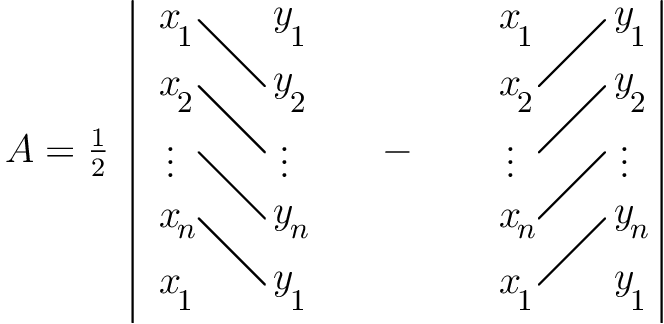
\includegraphics[width=0.45\linewidth]{schoelace}
\end{figure}
the resulting image looks like laced-up shoes.

This can also be written in form of a summation
\begin{equation}
A = \dfrac{1}{2} \left|\sum_{i=1}^n{(x_{i+1}+x_i)(y_{i+1}-y_i)}\right|
\end{equation}
or in terms of determinants as
\begin{equation}
A = \dfrac{1}{2} \left|\sum_{i=1}^n{\det\begin{pmatrix}x_i&x_{i+1}\\y_i&y_{i+1}\end{pmatrix}}\right|
\end{equation}
which is useful in the $3D$ variant of the Shoelace theorem. Note here that $x_{n+1} = x_1$ and $y_{n+1} = y_1$.

The formula may also be considered a special case of Green's Theorem
\begin{equation}
\tilde{A}=\int \int \left(\frac{\partial M}{\partial x}-\frac{\partial L}{\partial y}\right)dxdy=\oint(Ldx+Mdy)
\end{equation}
where $L=-y$ and $M=0$ so $\tilde{A}=A$.

\subsubsection{Proof}
\paragraph{Claim 1} The area of a triangle with coordinates 
$A(x_1, y_1)$, $B(x_2, y_2)$, and $C(x_3, y_3)$ is
\begin{equation}
\cfrac{|x_1y_2+x_2y_3+x_3y_1-x_1y_3-x_2y_1-x_3y_2|}{2}
\end{equation}

\paragraph{Proof of Claim 1} Writing the coordinates in 3D and translating $\triangle ABC$ so that $A=(0, 0, 0)$ we get the new coordinates $A'(0, 0, 0)$, $B(x_2-x_1, y_2-y_1, 0)$, and $C(x_3-x_1, y_3-y_1, 0)$. Now if we let $\vec{b}=(x_2-x_1 \quad y_2-y_1 \quad 0)$ and $\vec{c}=(x_3-x_1 \quad y_3-y_1 \quad 0)$ then by definition of the cross product

\begin{equation}
[ABC]=\frac{||\vec{b} \times \vec{c}||}{2}=\frac{x_1y_2+x_2y_3+x_3y_1-x_1y_3-x_2y_1-x_3y_2}{2}
\end{equation}

\paragraph{Proof} We will proceed by induction. By claim 1, the shoelace theorem holds for any triangle. We will show that if it is true for some polygon $A_1A_2A_3...A_n$ then it is also true for $A_1A_2A_3...A_nA_{n+1}$.

We cut $A_1A_2A_3...A_nA_{n+1}$ into two polygons, $A_1A_2A_3...A_n$ and $A_1A_nA_{n+1}$. Let the coordinates of point $A_i$ be $(x_i, y_i)$. Then, applying the shoelace theorem on $A_1A_2A_3...A_n$ and $A_1A_nA_{n+1}$ we get

\begin{align}
A_{n} &= [A_1A_2A_3...A_n] =\frac{1}{2}\sum_{i=1}^{n}(x_iy_{i+1}-x_{i+1}y_i) \\
A_{n+1} &= [A_1A_nA_{n+1}] =\frac{1}{2}(x_1y_2+x_2y_3+x_3y_1-x_1y_3-x_2y_1-x_3y_2)
\end{align}

Hence
\begin{equation}
\begin{gathered}
 A = A_{n+1} + A_n =\frac{1}{2}\sum_{i=1}^{n}(x_iy_{i+1}-x_{i+1}y_i)+\frac{1}{2}(x_1y_2+x_2y_3+x_3y_1-x_1y_3-x_2y_1-x_3y_2)\\ =\frac{1}{2}((x_2y_1+x_3y_2+...+x_{n+1}y_n+x_1y_{n+1})-(x_1y_2+x_2y_3+...+x_ny_{n+1}+x_{n+1}y_1))\\
 =\boxed{\frac{1}{2}\sum_{i=1}^n(x_iy_{i+1}-x_{i+1}y_i)}
\end{gathered}
\end{equation}
as claimed.
\subsection{Pick Theorem}

\emph{Pick's Theorem} states that if a polygon has vertices with integer coordinates (\emph{lattice points}) then the area of the polygon is 
\begin{equation}
F(P) = area(P) - \left(i + \cfrac{1}{2}\cdot p - 1\right)
\end{equation}
where $i$ is the number of lattice points inside the polygon and $p$ is the number of lattice points on the perimeter of the polygon.

\paragraph{Proof} To prove Pick's Theorem, we have to show that this function takes the value zero for all planar polygons. You will need to use the fact that any polygon can be split into a finite number of non-overlapping triangles.

The sequence of five steps in this proof starts with \emph{adding} polygons by glueing two polygons along an edge and showing that if the theorem is true for two polygons then it is true for their \emph{sum} and \emph{difference}.

The next step is to prove the theorem for a rectangle, then for the triangles formed when a rectangle is cut in half by a diagonal, then for the general triangle (labelled $T$ in the diagram below), and finally for any planar polygon because it can be built up from \emph{adding} triangles. Although the proof is long it is simply a matter of counting points.

\begin{enumerate}
\item Let $P_1$ and $P_2$ be non-overlapping polygons that abut along a common edge $AB$. Let $P$ be the union of $P_1$ and $P_2$ and $i$, $i_1$ and $i_2$ the lattice points inside and $p$, $p_1$ and $p_2$ the lattice points on the perimeter of $P$, $P_1$ and $P_2$ respectively. Prove that if Pick's function is zero for any two of these polygons it must be zero for the third.
\item Prove that Pick's function is zero for the rectangle with vertices $(0,0)$, $(a,0)$, $(0,b)$ and $(a,b)$ where $a$ and $b$ are integers.
\item Two triangles are produced when the rectangle with vertices $(0,0)$, $(a,0)$, $(0,b)$ and $(a,b)$ is cut in half by one or other of the diagonals. Prove that Pick's function is zero for these triangles and hence that Pick's Theorem holds for any right-angled triangle with sides parallel to the axes.
\item Prove that Pick's Theorem holds for the general triangle $T$ shown in this diagram. 
\item Prove that Pick's Theorem holds for any planar polygon.
\end{enumerate}

\begin{figure}[htbp]
\centering
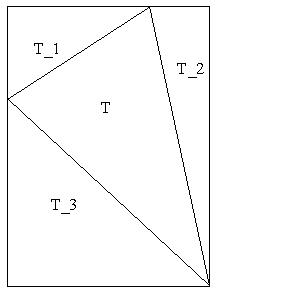
\includegraphics[width=0.45\linewidth]{pick_theorem}
\end{figure}

\subsection{Day XX - }
\subsubsection{Lagrange polynomial}

\subsection{Day 12 - Dynamic Programming}
Dynamic Programming (memoization)

\subsection{Hanlon's razor}

Hanlon's razor is an adage or rule of thumb that states:

\vspace*{\fill} 
\begin{quote} 
	\centering 
	"Never attribute to malice that which is adequately explained by stupidity."
\end{quote}
\vspace*{\fill}

It is a philosophical razor that suggests a way of eliminating unlikely explanations for human behavior. Similar statements have been recorded since at least the 18th century. The adage was a submission credited in print to Robert J. Hanlon of Scranton, Pennsylvania, in a compilation of various jokes related to Murphy's law that were published in Arthur Bloch's Murphy's Law Book Two: More Reasons Why Things Go Wrong! (1980).

A similar quotation appears in Robert A. Heinlein's novella Logic of Empire (1941). The character "Doc" in Heinlein's story described the "devil theory" fallacy, explaining, "You have attributed conditions to villainy that simply result from stupidity."

Hanlon's razor became well known after its inclusion in the Jargon File, a glossary of computer programmer slang, since 1990. Later that same year, the Jargon File editors noted lack of knowledge about the term's derivation and the existence of a similar epigram by William James, although this was possibly intended as a reference to William James Laidlay. In 1996, the Jargon File entry on Hanlon's Razor noted the existence of the phrase in Heinlein's novella, with speculation that Hanlon's Razor might be a corruption of "Heinlein's Razor". 

The name was inspired by Occam's razor.

\subsection{Day 14 - Parabolic Reflector Dish}

\subsubsection{List of \texttt{numpy.array}}

It is not straightforward to look for a \verb|numpy.array| into a list. The following functions are useful to get either the \verb|array| index in the list or a boolean if the \verb|array| is in the list.

\begin{ipython}
import numpy as np

def arreq_in_list(myarr, list_arrays):
    return next((True for elem in list_arrays 
                 if np.array_equal(elem, myarr)), False)

def arridx_in_list(myarr, list_arrays):
    return next((i for i, elem in enumerate(list_arrays) 
                 if np.array_equal(elem, myarr)), -1)
\end{ipython}

\end{document}
